\section{Wstęp}
    Celem poniższej pracy jest zbudowanie autonomicznego pojazdu, 
    którego zadaniem będzie zbudowanie wirtualnej mapy terenu.
    Użytkownik powinien mieć możliwość za pomocą dedykowanej aplikacji komputerowej zobaczyć mapę zbudowaną przez poszczególne urządzenia.
    Na przedstawionej mapie móc wybrać punkt docelowy. 
    Następnie samochód powinien zaproponować optymalną trasę, którą będzie podążał.


    \subsection{Środowisko sprzętowe}
        Współczesne pojazdy autonomiczne wyposażone są w olbrzymie jednostki obliczeniowe, bardziej swoją konstrukcją przypominające pełnoprawne komputery z systemem operacyjnym.
        Ten projekt ma być tylko modelem, pozwalajacym przedstawić zachowanie pojazdu autonomicznego, dlatego wykorzystanie pełnoprawnego komputera wydaje się być zbędne.

        \subsubsection{Mikrokontroler}
            Poniżej przedstawiono kilka najbardziej popularnym platform sprzętowych, które mogą stanowić bazę dla samochodu.
            \begin{enumerate}
                \item Raspberry Pi -- pełnoprawny komputer z systemem operacyjnym Linux, umożliwiający bezpośredni dostęp do modułów zewnętrznych z pomocą GPIO.
                Jest to najbardziej popularna platforma dla projektów DIY. System wraz z peryferiami komputerowymi pozwala na niesamowitą elastyczność w pracy, między innymi na połączenie się do układu za pośrednictwem SSH oraz pracę w języku Python.
                Jednak ze względu na swoją popularność, jest bardzo drogi i mało dostępny. 
                A zaleta jaką jest system operacyjny jest też wadą gdy chcemy aby nasz projekt działał w czasie rzeczywistym.
                \item Arduino -- najpopularniejszy mikrokontroler, którego największą zaletą jest prostota framework'a Arduino oraz mnogość bibliotek do każdego układu.
                Niestety, płytki te operate są o 8-bitowe mikrokontrolery z rodziny AVR, co sprawia, że są bardzo wolne (max 20MHz). 
                Sam framework wykorzystywany jest na wielu różnych praformach, przez co jego szybkość jest dyskusyjna.
                \item STM32 -- układu projektowane przez firmę STMicroelectronics, które są znacznie szybsze od Arduino, a także mają znacznie więcej pamięci.
                Jednak środowisko programistyczne \textit{STM Cube IDE}, czy biblioteka HAL sprawiają, że programowanie jest znacznie trudniejsze w porównaniu do innych układów.
                \item ESP32 -- 32-bitowy dwurdzeniowy procesor z wbudowanym modułem WiFi i Bluetooth.
                Jeden z najszybszych mikrokontrolerów na rynku, który jest bardzo popularny w projektach IoT.
                Natywnie pracuje pod kontrolą systemu czasu rzeczywistego FreeRTOS, co sprawia, że może być idealnym kandydatem do tego projektu.
                Jednak bardzo słaba dokumentacja, dyskredytują go w oczach wielu programistów.
                \item Raspberry Pi Pico -- mikrokontroler od firmy Raspberry Pi, który jest znacznie szybszy od Arduino $f_{cpu} = 125MHz$.
                Ma znacznie więcej pamięci $2MB$ w porównaniu z Arduino~$32KB$.
                Producent udostępnił wyjątkowo estetyczne SDK w języku C, do którego przygotował masę przykładów.
                Sama dokumentacja jest stale rozwijana i wprowadzane są nowe poprawki.\\
                W roku 2022, pojawiła się druga iteracji tej płytki rozwojowej z dopiskiem ,,W" (Pico~W), która posiada wbudowany moduł WiFi.
            \end{enumerate}
            Wszystkie wymienione platformy są w stanie zrealizować projekt, jednak ze względu na swoją prostotę, Raspberry Pi Pico wydaje się być najlepszym wyborem.

        \subsubsection{Sterowanie}
        \label{sec:engines}
            Podstawowym zadaniem samochodu jest możliwość jazdy, niezwykle kluczowe jest wybranie odpowiedniego silnika napędowego.
            Na rynku konsumenckim dostępnych jest wiele różnych wariantów, poniżej opisano możliwe opcje.
            \begin{enumerate}
                \item Silniki krokowe -- kiedyś bardzo duże i drogie silniki, które potrzebowały dodatkowych układów sterowania. 
                Dziś jednak istnieją małe $5V$ rozwiązania, które moga być sterowanie bezpośrednio przez mikroprocesor.
                Jednak złożone sterowanie, oraz mała prędkość maksymalna $v_{max} \approx 1 \frac{\text{obr.}}{s}$ eliminują ten rodzaj silników.
                \item Serwomechanizmy $360^\circ$ -- serwomechanizmy to układ silnika wraz z kontrolerem prędkości oraz przekładniami, sterowanie takimi silnikiem pozwala na ustawienie bardzo dokładnej wartości prędkości dla każdego silnika.
                Jednak nie istnieje żadna możliwość, sprawdzenia czy serwo A oraz drugie serwo B, pracują z tą samą prędkością. Co może prowadzić do wielu nie przewidzianych zachowań, na przykład znoszenie pojazdu w jedną stronę.
                \item Serwomechanizmy $180^\circ$ -- odmiana serwomechanizmów pozwalająca na dosyć precyzyjne ustawienie żądanego kąta. 
                Układy nie nadają się do napędzania pojazdów, jednak świetnie odnajdują w sytuacjach gdy trzeba ustawić zadany kąt, na przykład podczas skręcania.
                \item Silniki BLDC -- najmocniejsze silniki, pozwalające osiągnąć nieporównywalne prędkości.
                Niestety same silniki nie należą do tanich, a dodatkowo każdy silnik wymaga specjalistycznego układu sterującego.
                \item Silniki DC -- proste, tanie silniczki prądu stałego, pozwalające na regulację prędkości za pomocą PWM. 
                Dodatkowo w sprzedaży dostępne są układy wyposazone w enkodery, pozwalające obliczyć średnią szybkość silnika, 
                a także wyznaczyć różnicę w prędkościach pracy silników.
            \end{enumerate}
            Z powyższych rodzajów silników do napędu, najlepszymi wydają się silniki DC z zamontowanym enkoderem.
            Natomiast do układu kierowniczego, najlepiej nada się serwomechanizmy $180^\circ$. Oba wybrane układy przedstawiono na zdjęci \ref{fig:engines} poniżej.
            \begin{figure}[!ht]
                \centering
                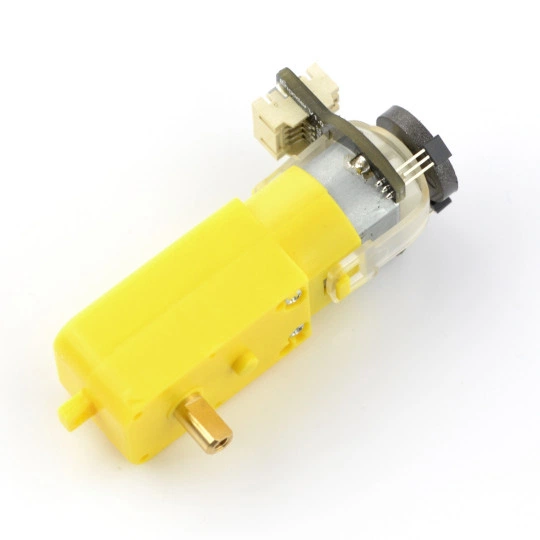
\includegraphics[width = 0.3\textwidth]{silnik_z_enkoder.png}
                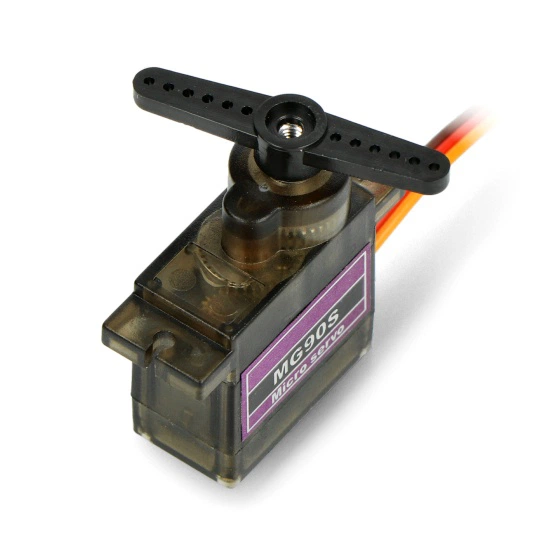
\includegraphics[width = 0.3\textwidth]{serwo_180.png}
                
                \caption{Silnik DC z enkoderem oraz serwomechanizmy $180^\circ$.}
                \footnotesize{Źródło: \href{https://botland.com.pl/}{botland.com}}
                % Źródło: https://botland.com.pl/silniki-dc-z-przekladnia-i-enkoderami/6287-silnik-z-przekladnia-sj01-120-1-6v-160rpm-enkoder-6959420910205.html
                % Źródło: https://botland.com.pl/serwa-typu-micro/20435-serwo-mg-90s-micro-180-stopni-metalowa-przekladnia-5904422380915.html
                \label{fig:engines}
            \end{figure}
        
        \subsubsection{Pomiar odległości}
            Pojazdy autonomiczne muszą być świadome swojego otoczenia, a do tego ważne jest aby były w stanie ocenić przynajmniej orientacyjną odległość od najbliższej przeszkody.
            Poniżej przedstawiono listę kilku rodzajów czujników, pozwalających określić odległości do najbliższych obiektów.
            \begin{enumerate}
                \item Czujnik ultradźwiękowy -- najtańsze układy do pomiaru odległości, bardzo prymitywne. O bardzo niestabilnym pomiarze.
                \item Czujniki Time of Flight (ToF) -- złożone wyspecjalizowane moduły pozwalające na dużą dokładność pomiarową oraz bardzo daleki zasięg.
                Zazwyczaj wymagają specjalnych bibliotek dostarczonych przez producenta
                \item Układy obiciowe IR -- proste dwu diodowe układy emitera i pomiaru natężenie światła podczerwonego. Układy o małej dokładności pomiarowej, dużej strefie martwej (old $2cm$ do $20cm$), małej stabilności pomiarowej. Pomiar zależy od koloru obiektu.
                \item Lidar -- drogie wyspecjalizowane układy, pozwalające na bardzo precyzyjny pomiar w pełnym zakresie $360^\circ$ w okół pojazdu.
                \item Radar -- bardzo drogie i bardzo dokładne układy pomiarowe, pozwalające na niezwykła precyzję. Niestety, praktycznie nie dostępne w względnie małych rozmiarach na rynku konsumenckim. Dodatkowo wymają specjalnych procesorów sygnałowych pozwalających w miarę na bieżąco przetwarzać dane z radarów.
            \end{enumerate}
            Z przedstawionej listy, najlepszym układem dla tego zastosowania, wydaje się czujnik typu ToF.
            Dodatkowo, w celach bezpieczeństwa z tyłu pojazdu zostały zamontowane czujniki IR, ale nie jako urządzenia pomiarowe, pozwalające zmierzyć odległość do przeszkody.
            Tylko jako czujniki zbliżeniowe, umożliwiające wykrycie przeszkody i zahamowanie przed zderzeniem.

    \subsection{Środowisko programistyczne}
        Następnym bardzo ważnym wyborem jest środowisko programistyczne, w którym zostanie zbudowany projekt.
        Tutaj też w ostatnich latach użytkownicy dostali możliwość obżymiego wyboru.
        Podstawowymi rozwiązaniami dla programistów embedded są
        \begin{enumerate}
            \item Eclipse -- kiedyś bardzo popularny, posiadający olbrzymi zbiór dodatków. 
            Jest także rozprowadzany na otwartej licencji dlatego stanowi świetną bazę dla wielu bardziej zaawansowanych projektów.
            \item STM32 Cube -- środowisko przeznaczone strike do pracy z modułami STM32, oparte na Eclipsie.
            \item Atmel Studio -- środowisko przeznaczone do pracy z mikrokontrolerami z rodziny AVR od firmy ATmel.
            \item Keil µVision -- środowisko ogólnego przeznaczenia do pracy z układami Cortex, ograniczone licencją oraz bardzo toporne w pracy.
            \item Notepad++ -- bardziej zaawansowany notatnik, pozwalający na auto uzupełnianie słów. Na też masę wtyczek, pozwalających na stworzenie z niego pełnoprawnego środowiska programistycznego, jednak w swojej pierwotnej wersji bardzo toporny w użyciu.
            \item VS Code -- bardzo uniwersalne narzędzie, mające olbrzymią masę dodatków, pozwalających przystosować środowisko w pełni pod własne wymagania.
            Samo środowisko jest zbudowane na silniku przeglądarki internetowej, dzięki czemu może z powodzeniem zastąpić przeglądarkę PDF, a w wbudowany tile menedżer pozwala układać całość w bardzo czytelny sposób.
        \end{enumerate}
        Projekt został, zbudowany w środowisku VS Code, ze względu na największą elastyczność oraz możliwość dostosowania go do własnych potrzeb.



    \subsection{Środowisko CAD}
        